\documentclass[openany]{article}
\usepackage[english]{babel}
\usepackage{commands}
\usepackage{xcolor}
\usepackage{caption}
\usepackage{subcaption}
\usepackage{graphics}
\usepackage{lipsum}

\pagestyle{fancy}
\fancyhf{}
\lhead{}
\rhead{\leftmark}
\cfoot{\thepage}

\usepackage{biblatex} %Imports biblatex package
\addbibresource{refs.bib}

\begin{document}

\counterwithout{equation}{section}

\thispagestyle{empty}    

\begin{titlepage}
\begin{figure}[th]
\begin{flushleft}
    
\includegraphics[width=7cm]{ugr.png}
\end{flushleft}
\end{figure}
 \vspace{1cm}

{\flushleft \LARGE \bfseries MASTER'S THESIS\par}\vspace{2cm}

% Thesis title
{\flushright \LARGE \bfseries Performance of a neural network model for
stereotactic radiosurgery with a dynamic micro-
multileaf collimator  \par}\vspace{2cm}

{\flushleft \LARGE \bfseries Armando Delgado Fumero \par}\vspace{1.5cm}

{\flushleft \bfseries Master’s Degree in Physics and Mathematics \par}\vspace{0.cm}

{\flushleft \small \bfseries Academic Year 2021/2022\par}
{\flushleft \small \bfseries Supervisors:
\begin{itemize}
    \item Luis Díaz Angulo (UGR)
    \item Wilfredo González (UMA)
\end{itemize}}\vspace{2cm}



\end{titlepage}

\clearpage\thispagestyle{empty}\null\newpage %blank page
	
\pagenumbering{arabic}


\newpage
\thispagestyle{plain}
{
\hypersetup{hidelinks}
\tableofcontents
}

\newpage 
\thispagestyle{empty}


\thispagestyle{plain}

\section{Abstract}

Based on the work of González (2015) \cite{Gonzalez2015}, our goal is to develop a neural network based solution that allow us to predict the fluence outcome of a 6 MV Elekta Precise linac. This project goes through two main steps, first, we use Fippel et al (2003) \cite{Fippel} VSM (Virtual Source Model) to get a first approximation to the data, obtaining needed coefficients using a MonteCarlo iteration method. Now, out of this analytic equation which approximates the fluence results, we train and test a Convolutional Neural Network, improving the results of the analytic function.

    \vspace{2cm}
    




\pagenumbering{arabic}

\newpage

\section{Introduction} \label{sec: introduction}

\subsection{Linac}


A linear acelerator (linac) is an artifact that uses microwave technology to initially accelerate electrons on a wave guide. These accelerated electrons hit a metal target, which produces x-rays. These photons product of the collision are directed towards the machine exit, shaped as the physician requires. These machines are used mainly on cancer treatments, delivering the radiation to the tumor.

\begin{figure}[!h]
    \centering
    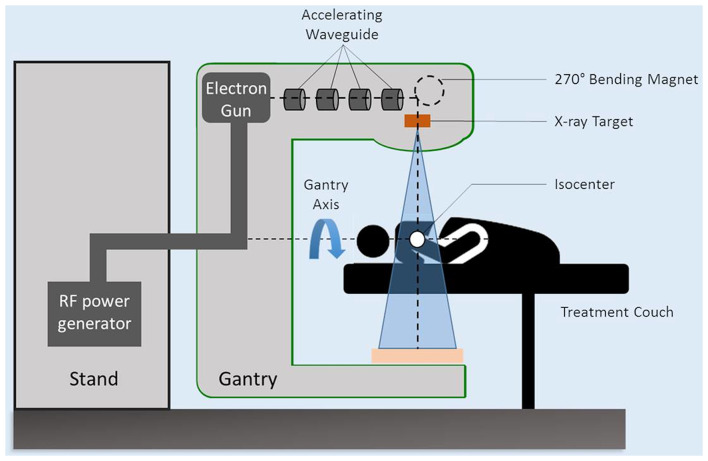
\includegraphics[width=\textwidth]{fcvm-07-00108-g0003.jpg}
    \caption{Schematic diagram of a linac \cite{Jumeau}}
    \label{fig:my_label}
\end{figure}





\subsection{Elekta MV 6}


\subsection{Dataset}

The data used in this work will be the product of a measuring of the radiation produced by the earlier mentioned Elekta MV 6 over a water mannequin, a quite common method when it comes to radiation procedures \cite{Lutz1984-ex}, \cite{BenitesR2012}, \cite{Gonzalez2015}, \cite{Tessonnier} . The result of these measurings is a total of 96 text files, each one of these correspond to a different combination of height, area and presence (or not) of a scattering part. We can see an example of one of these profiles on Figure 2. Text files shape are as shown on table 1.


\begin{figure}[!h]
    \centering
    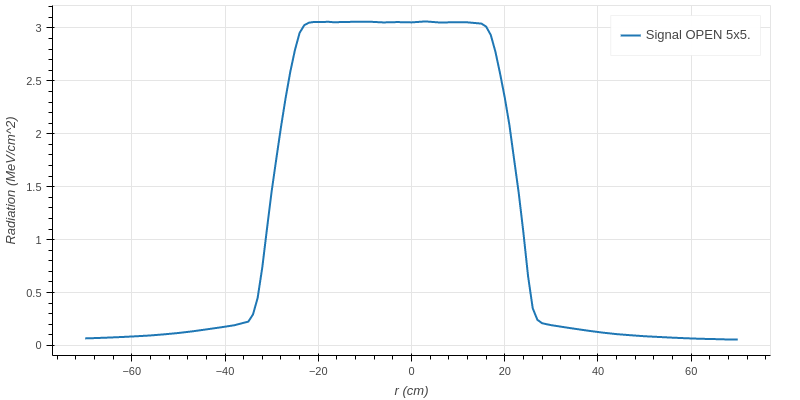
\includegraphics[width=\textwidth]{ProfileExample.png}
    \caption{5x5 open profile on y axis, z=100cm}
    \label{fig:my_label}
\end{figure}


\begin{table}[!h]
    \centering
\begin{tabular}{lrrr}
\toprule
{} &     \textbf{r} &  \textbf{señal open 5x5} &  \textbf{error open 5x5} \\
\midrule
\hline
\hline

0 & -70.0 &        0.066602 &         0.31080 \\
1 & -68.0 &        0.069431 &         0.31110 \\
2 & -65.0 &        0.074360 &         0.31065 \\
3 & -62.0 &        0.080116 &         0.31080 \\
4 & -59.0 &        0.086831 &         0.31095 \\
... & ... & ... & ... \\
70 &  59.0 &        0.067845 &         0.31395 \\
71 &  62.0 &        0.063037 &         0.31410 \\
72 &  65.0 &        0.060057 &         0.31470 \\
73 &  68.0 &        0.056351 &         0.31410 \\
74 &  70.0 &        0.055396 &         0.31410 \\
\hline
\hline

\bottomrule
\end{tabular}
\caption{Example of 5x5 profile txt}
    \label{tab:my_label}
\end{table}

\newpage 

The files in this dataset comprise of all these possible combinations:

\begin{itemize}
    \item \textbf{Area}: 5x5, 5x40, 10x10, 10x40, 20x20, 40x5, 40x10, 40x40
    \item \textbf{Z}: 85, 100, 115
    \item \textbf{FFF (scatter)}: FFF, OPEN
\end{itemize}


\newpage 

\subsection{Goals}

So, this study was focused on obtaining a Virtual Source Model for this linac based on the dataset we do have. Previous models (\cite{BenitesR2012}, \cite{Gonzalez2015}, \cite{Tessonnier}, \cite{10.1007/978-3-642-21198-0_318}, \cite{phdthesis}, \cite{https://doi.org/10.1120/jacmp.v16i1.4992}, \cite{GONZALEZ201716}) have been centered on obtaining an analytic equation that is able to mathematically define the reality. They rely on MonteCarlo or similar methods to obtain coefficients for the equation, however, this may be not the fastest nor the most effective method to obtain these results. With the current expansion of Artificial Intelligence and bayesian statistics, it may be interesting to look up those methods to solve this problem. Our objective however will be mixed. On one hand, we will obtain an analytic equation that defines our problem, obtaining the needed coefficients via MonteCarlo. \\

Once we have solved that part, we will look to improve the current result of the analytic equation feeding that data as input to several Neural Networks, which will try to create a prediction. Using Neural Networks in medical physics is not something new, as it is widely used in cancer recognition \cite{BOTTACI1997469} \cite{Ganesan} \cite{Shen2019}. However, there are not many examples of its use on dosimetry \cite{G_tz_2020} \cite{Jiang} \cite{Lee2019} and most of them are quite new. As said on Lee et al., 2019 \cite{Lee2019}, "The direct Monte Carlo simulation is considered as a state-of-art voxel-based dosimetry technique; however, it incurs an excessive computational cost and time. To overcome the limitations of the direct Monte Carlo approach, we propose using a deep convolutional neural network (CNN) for the voxel dose prediction". However, we mix both methods, trying to obtain best from both worlds.

\newpage
\numberwithin{equation}{section}

\section{Analytic approximation}


Following Fippel et al (2003) \cite{Fippel} and González (2015) \cite{Gonzalez2015} VSMs, we develop one for this linac.

We can describe it as a two part equation, where the first leg of the equation corresponds to the main collimator and the second leg to the scattering. 

\begin{equation}
    \centering
    \Phi_\gamma (x,y,z) = w_0 \Phi_0(x,y,z) \Phi_{horn}^\gamma (x,y,z) + (1-w_0)\Phi_s(x,y,z) 
\end{equation}



Being more concise, \(w_0\) is the fraction of the contribution from the primary (and therefore, 1 minus \(w_0\) is the contribution from the scatter source), a normalized value. Then, \(\Phi_0\) and \(\Phi_s\) are the fluence equations for both collimator and scatter source. Finally, \(\Phi_{horn}\) is an equation that tries to define the central depression that we can see on the mayority of profiles. An example of this kind of profile can be seen on Figure 3.\\



\subsection{Photon Primary Source Fluence}

Fluence equations are defined as it follows:

\begin{equation}
    \centering 
    \Phi_\alpha = Z(z; z_D^x, z_D^y, z_\alpha) T_\alpha(x_\alpha^+, x_\alpha^-) T_\alpha(y_\alpha^+, y_\alpha^- )
    
\end{equation}

Out of these variables, Z (Eq 3.3) defines the reduction of the fluence based on the distance from the target to the source, while T defines the area. 

\begin{equation}
    \centering 
    Z(z; z^x_D, z^y_D, z_\alpha) = \frac{1}{4} \frac{(z_D^x - z_\alpha) (z^y_D - z_\alpha )}{(z-z_\alpha)^2}
    
\end{equation}

Now, T refer to x or y, depending on what axis are we on, and it is defined by Pearson VII equation (3.4). This Pearson VII equation with X and Y as subject, with \( \frac{t_0^\pm}{\delta_0}\) being \(v\), as shown on equation (3.5). So, X and Y would be defined by equations (3.6) and (3.7). 

\begin{equation}
    Q_0(v) = \frac{v}{\sqrt{1+v^2}} 
\end{equation}

\begin{equation}
    T_0 (\frac{t_0^\pm}{\delta_0}) = \frac{\frac{t_0^\pm}{\delta_0}}{\sqrt{1 + (\frac{t_0^\pm}{\delta_0})^2}}
\end{equation}


\begin{equation}
    \centering 
    X_0 = \frac{\frac{x_0^+}{\delta_0}}{\sqrt{1+\frac{x_0^+}{\delta_0}}} + \frac{\frac{x_0^-}{\delta_0}}{\sqrt{1+\frac{x_0^-}{\delta_0}}} \\
\end{equation}
\begin{equation}
    \centering 
    Y_0 = \frac{\frac{y_0^+}{\delta_0}}{\sqrt{1+\frac{y_0^+}{\delta_0}}} + \frac{\frac{y_0^-}{\delta_0}}{\sqrt{1+\frac{y_0^-}{\delta_0}}}
\end{equation}

Variables on this equation need some explanation as well. \(x_0^+\), \(x_0^-\), \(y_0^+\), \(y_0^-\) are the outer bounds that delimit the collimation area. They are defined in equation (3.9).

\begin{equation}
    t_\alpha^{\pm}  = min[\frac{w_I^tz_U^t(z-z_0) \pm 2t*z_I(z_0 - z_U^t)}{2z_I(z-z_U^t)}, \frac{w_I^tz_D^t(z-z_0) \pm 2xz_I (z_0-z_D^t)}{2z_I(z-z_D^t)}]
\end{equation}


\newpage


Now, we have finished defining new variables and these are actual data, being:

\begin{itemize}
    \item \(w_I^t\): Field size on the 'T' direction. 
    \item \(z_U^t\): and \(z_D^t\): "Up" and "Down" limits of the collimation system for x and y directions.
    \item \(z\): Position of the target on the \(z\) axis
    \item \(z_0\): Position of the main fluence source
    \item \(t\): Coordinate on x or y direction 
    \item \(z_I\): Z coordinate of the isocenter, which in this case is always 100.

    
\end{itemize}



Thereby, the photon primary source is defined in equation 3.8 (without incorporating the last definitios):

\begin{equation}
    \Phi_0 = \frac{1}{4} (\frac{(z_D^x - z_\alpha) (z^y_D - z_\alpha )}{(z-z_\alpha)^2})*(\frac{\frac{x_0^+}{\delta_0}}{\sqrt{1+\frac{x_0^+}{\delta_0}}} + \frac{\frac{x_0^-}{\delta_0}}{\sqrt{1+\frac{x_0^-}{\delta_0}}}) * (\frac{\frac{y_0^+}{\delta_0}}{\sqrt{1+\frac{y_0^+}{\delta_0}}} + \frac{\frac{y_0^-}{\delta_0}}{\sqrt{1+\frac{y_0^-}{\delta_0}}})
\end{equation}

\subsection{Central depression correction}

Since most profiles present a central depression on the signal, this is an added correction to the main fluence equation.

\begin{equation}
    \Phi_{horn}(x,y,z) = 1+ \rho^2 \sum_{k=0}^4 h_k \rho^k
    
\end{equation}

The so-called central depression is shown on Figure 3.

\begin{figure}[!h]
    \centering
    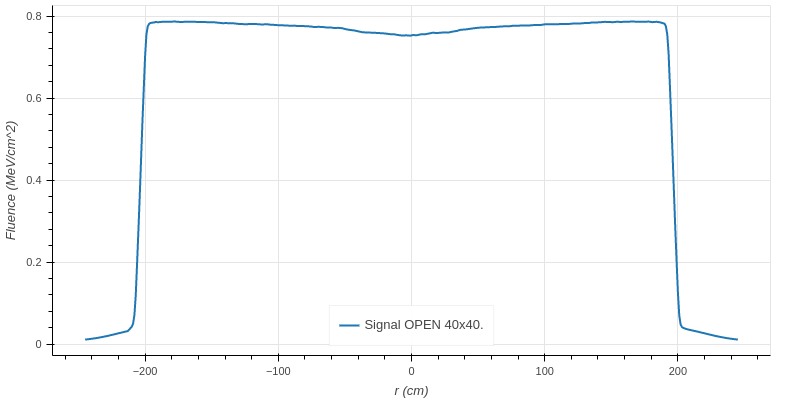
\includegraphics[width=\textwidth]{Central_Depression.png}
    \caption{'x' axis profile on the 40x40, Z=100..Central depression is more clear the larger the area is.}
    \label{fig:my_label}
\end{figure}

Where \(h_k\) are coefficients to obtain and \(\rho\) is a measure of the distance covered by the radiation:

\begin{equation}
    \rho = \frac{\sqrt{x^2 + y^2}}{z-z_0}
\end{equation}




Now, in cases where we only have the main fluence source \(w_0 = 1\) would be defined like:

\begin{equation}
    \Phi_\gamma = \frac{1}{4} (\frac{(z_D^x - z_\alpha) (z^y_D - z_\alpha )}{(z-z_\alpha)^2})*(\frac{\frac{x_0^+}{\delta_0}}{\sqrt{1+\frac{x_0^+}{\delta_0}}} + \frac{\frac{x_0^-}{\delta_0}}{\sqrt{1+\frac{x_0^-}{\delta_0}}}) * (\frac{\frac{y_0^+}{\delta_0}}{\sqrt{1+\frac{y_0^+}{\delta_0}}} + \frac{\frac{y_0^-}{\delta_0}}{\sqrt{1+\frac{y_0^-}{\delta_0}}}) * ( 1+ \rho^2 \sum_{k=0}^4 h_k \rho^k)
\end{equation}


To find these coefficients, we iterate our equation through a list of values, comparing all our signals to the results of the equations until we find the closest one. Results obtained are similar to the one showed on Figure 3. 

\begin{figure}[!h]
    \centering
    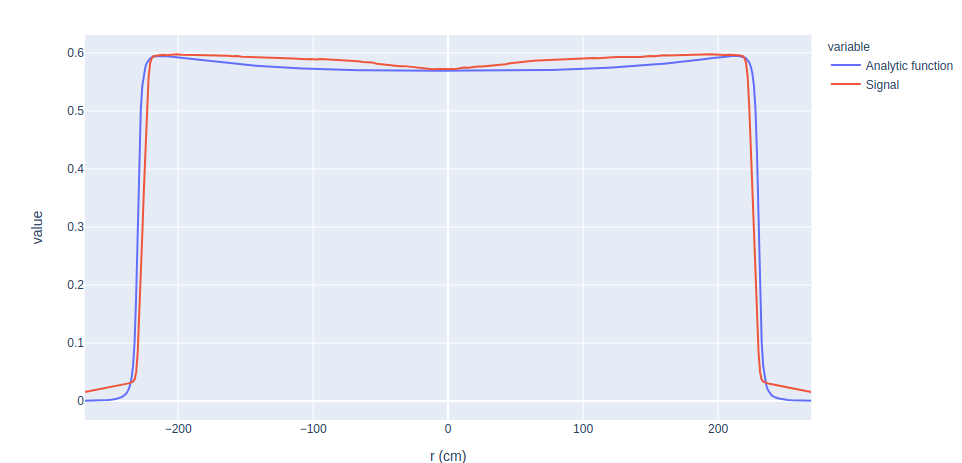
\includegraphics[width=15cm]{Limit400Z115.png}
    \caption{Signal and Analytic Function fitted using a 3 coefficient equation as \(\Phi_{horn}\). This is the plotting of a case where there is no scatter signal, Z=115 and the area to be covered is 40x40 cm}
    \label{fig:my_label}
\end{figure}


\subsection{MonteCarlo method}







\newpage

\section{Artificial Intelligence}


Now, Analytic functions are great, but we can see on Figure 2 that the central depression is not regular nor entirely symetrical. To adress these imperfections product of a real environment with an analytical function we would need to add more variables to an already intrincated equation, and not even after tha we would probably get an accurate definition. To solve this problem we propose an alternate way to achieve this result, using neural networks. Machine learning is a vast field of investigation these days due to their kinda "user-friendly" environment, being mayority of big tech companies creating their own machine learning suites. Machine learning is basically mathematic algorithms such as random forests or gradient boosting that are fitted to training data and then try to predict over a test data. For that purpose, we separate the data in 'x' and 'y', being 'x' the variables we are using to obtain an output, that is y. Algorithm learns from a training data of both 'x' and 'y', and then, once the algorithm is modelled, makes a 'y\_test' prediction based on the 'x\_test' data. Usually, algorithms will iterate through many tries to obtain the best try.

\begin{figure}[ht]
\begin{subfigure}
  \centering
  % include first image
  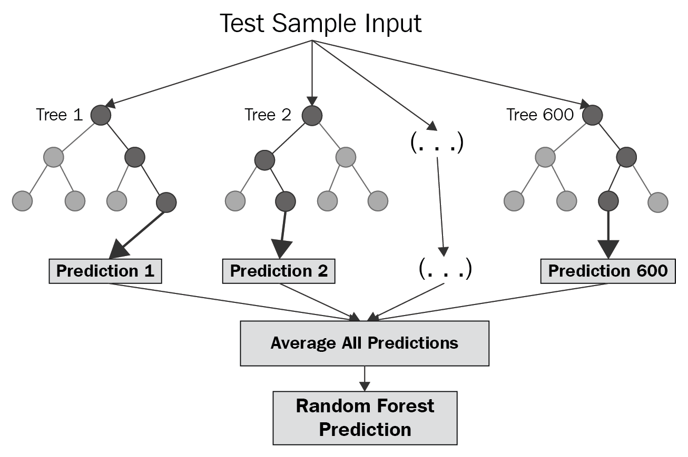
\includegraphics[width=5cm]{random-forest.png}  
  \caption{Random Forest}
  \label{fig:sub-first}
\end{subfigure}
\begin{subfigure}
  \centering
  % include second image
  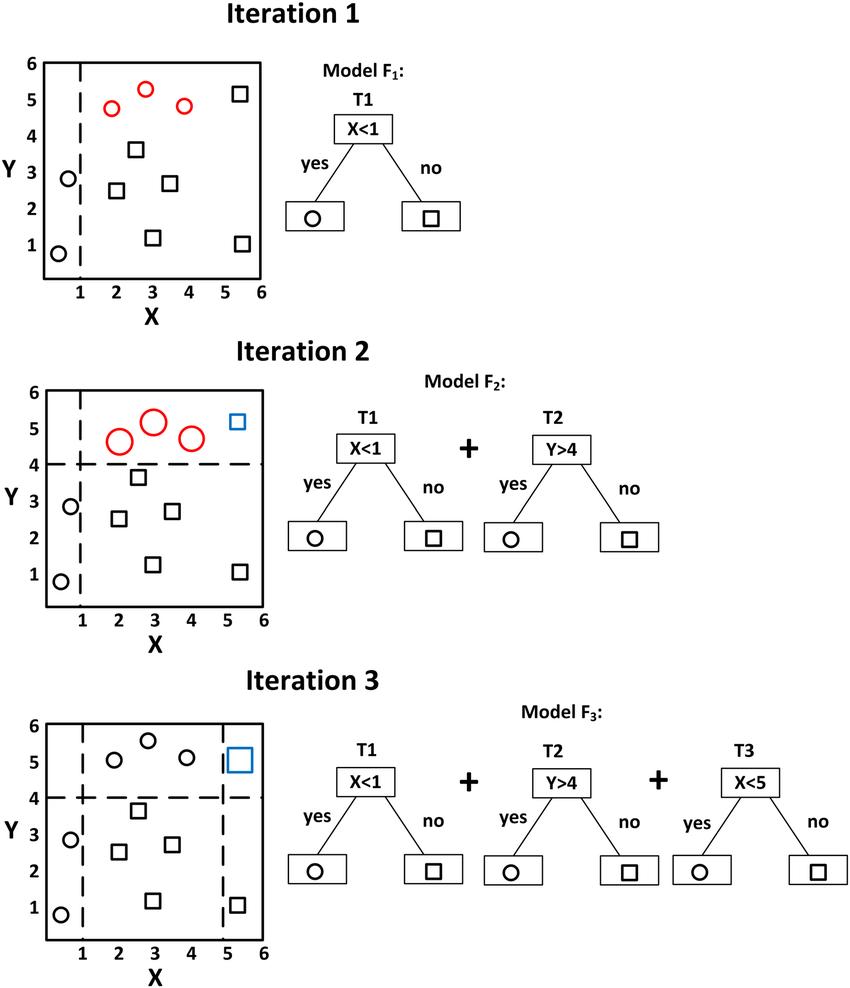
\includegraphics[width=5cm]{A-simple-example-of-visualizing-gradient-boosting.png}  
  \caption{Gradient Boosting}
  \label{fig:sub-second}
\end{subfigure}
\caption{Despite they may look the same there's a difference, random forest builds many trees independently and at the end does an average between the results. Gradient Boosting is an additive model that makes new trees depending on the result, doing the average along the way}
\label{fig:fig}
\end{figure}



\subsection{Neural Networks}

Neural Networks is the latest installment on AI. 


\subsection{Convolutional Neural Networks}
\newpage
\section{Results} \label{sec: numerical_results}

\subsection{Results I}

    \lipsum[2]

\subsection{Results II}

    \lipsum[2]

\subsection{Results III}

    \lipsum[2]
    
\subsection{Results IV}

    \lipsum[2]
    
    
    
    

\newpage
\section{Model validation}

   \lipsum[5]
    
    

\newpage
\section{Conclusions}

    \lipsum[4]
\newpage

\newpage

\newpage

\printbibliography

\newpage



\end{document}